\hypertarget{time-to-first-response}{%
\subsubsection{Time to First Response}\label{time-to-first-response}}

Question: How much time passes between when an activity requiring
attention is created and the first response?

\hypertarget{description}{%
\paragraph{Description}\label{description}}

The first response to an activity can sometimes be the most important
response. The first response shows that a community is active and
engages in conversations. A long time to respond to an activity can be a
sign that a community is not responsive. A short time to respond to an
activity can help to engage more members into further discussions and
within the community.

\hypertarget{objectives}{%
\paragraph{Objectives}\label{objectives}}

Identify cadence of first response across a variety of activities,
including PRs, Issues, emails, IRC posts, etc. Time to first response is
an important consideration for new and long-time contributors to a
project along with overall project health.

\hypertarget{implementation}{%
\paragraph{Implementation}\label{implementation}}

Time to first response of an activity = time first response was posted
to the activity - time the activity was created.

\hypertarget{filters}{%
\subparagraph{Filters}\label{filters}}

\begin{itemize}
\tightlist
\item
  Role of responder, e.g., only count maintainer responses
\item
  Automated responses, e.g., only count replies from real people by
  filtering bots and other automated replies
\item
  Type of Activity, e.g., issues (see metric
  \href{https://github.com/chaoss/wg-evolution/blob/master/metrics/Issue_Response_Time.md}{Issue
  Response Time}), emails, chat, change requests
\end{itemize}

\hypertarget{visualizations}{%
\subparagraph{Visualizations}\label{visualizations}}

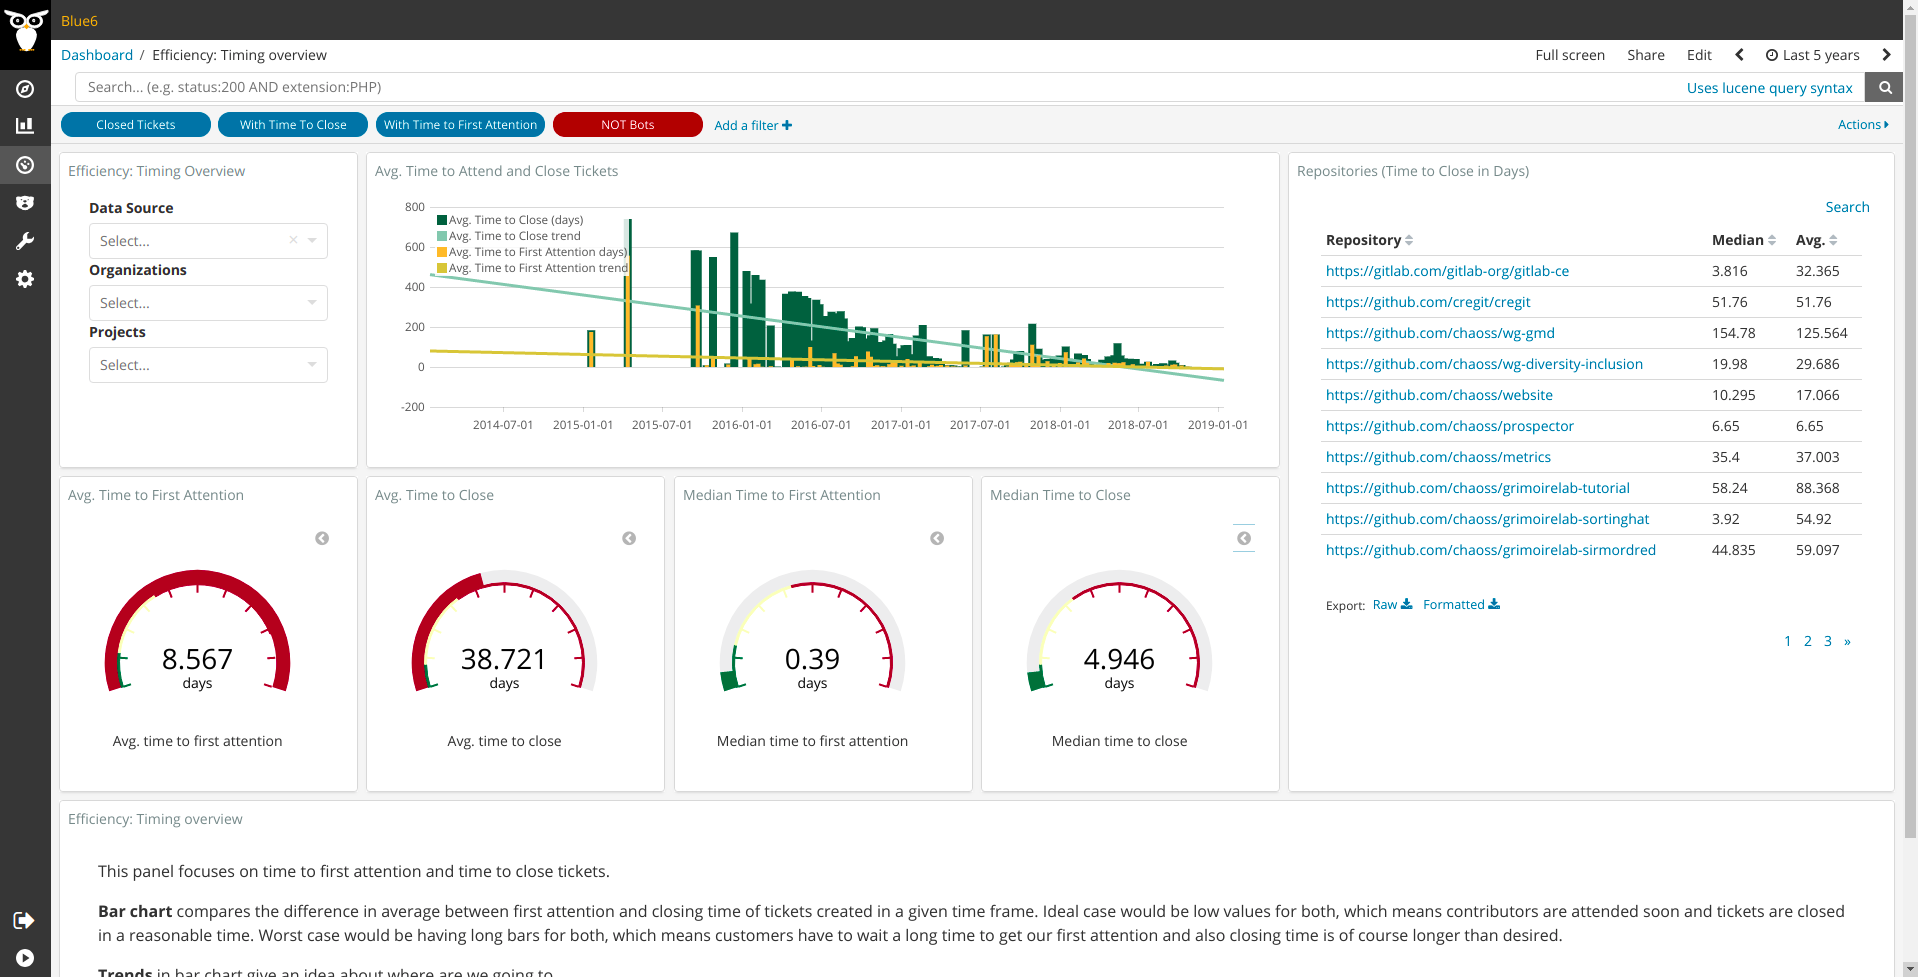
\includegraphics{images/time-to-first-response_efficiency-timing-overview.png}

\begin{center}\rule{0.5\linewidth}{0.5pt}\end{center}

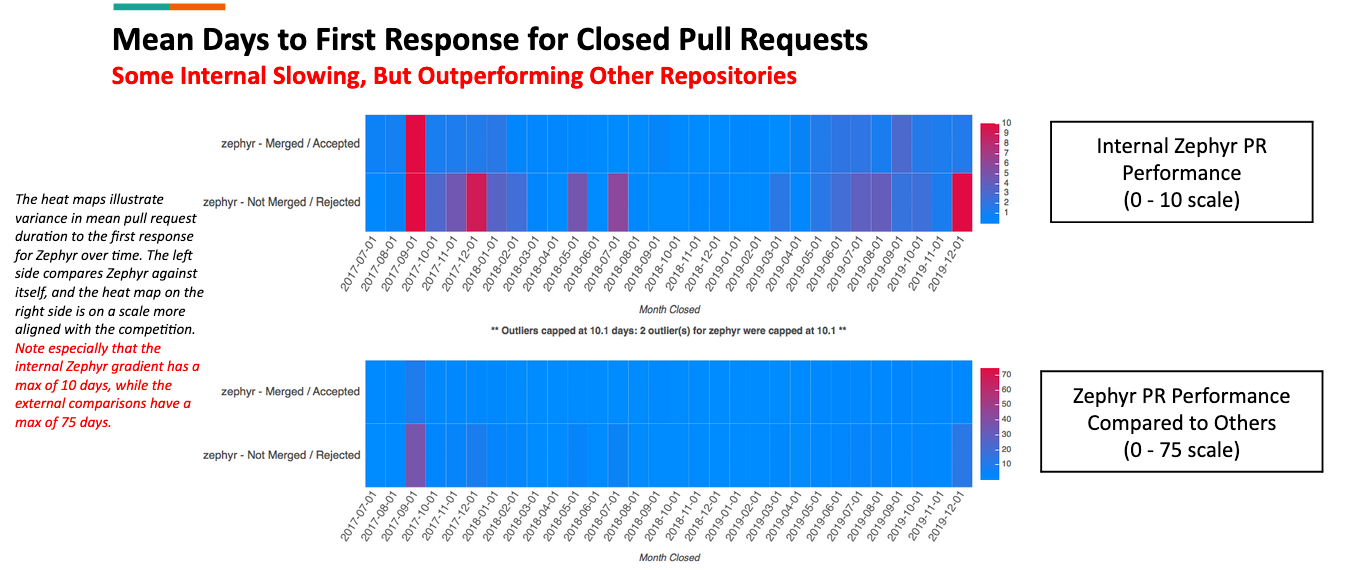
\includegraphics{images/time-to-first-response_augur-ttc-1.png}

\begin{center}\rule{0.5\linewidth}{0.5pt}\end{center}

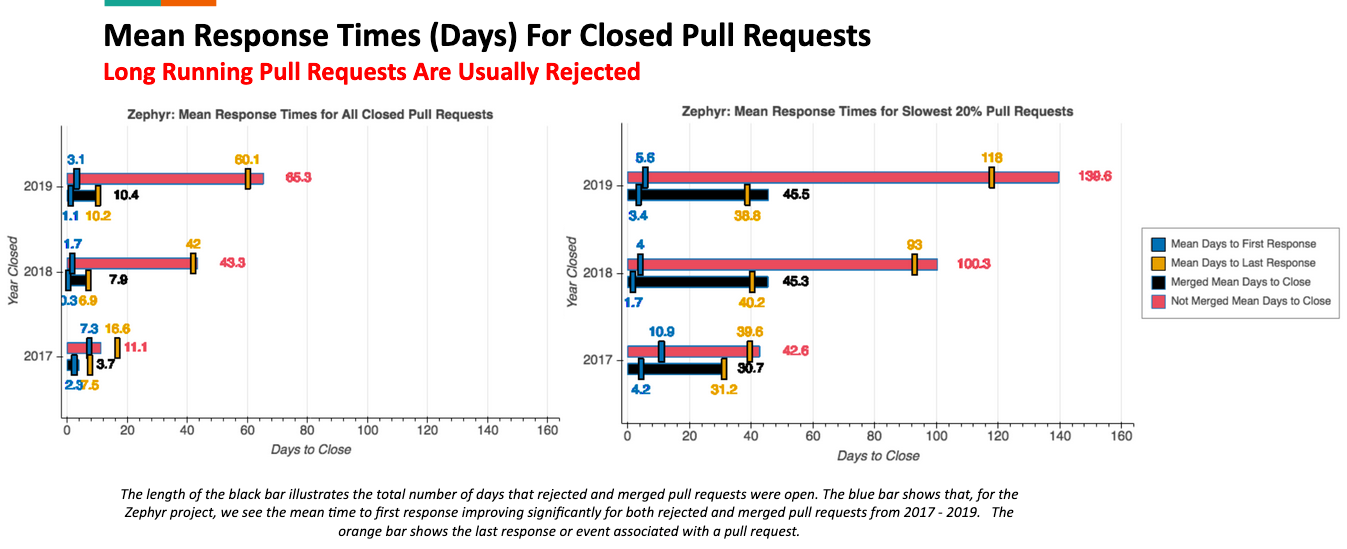
\includegraphics{images/time-to-first-response_augur-ttc-2.png}

\hypertarget{tools-providing-the-metric}{%
\subparagraph{Tools Providing the
Metric}\label{tools-providing-the-metric}}

\begin{itemize}
\tightlist
\item
  GrimoireLab Panel:
  \href{https://chaoss.github.io/grimoirelab-sigils/panels/efficiency-timing-overview/}{Efficiency
  Timing Overview}
\item
  \href{https://katacontainers.biterg.io/app/kibana\#/dashboard/cbbdd920-288c-11e9-b662-975152e57997}{Kata
  Containers dashboard efficiency panel}
\end{itemize}

\hypertarget{references}{%
\paragraph{References}\label{references}}
